\documentclass[tikz,border=8pt]{standalone}
\usepackage{amsmath,amssymb}
\usetikzlibrary{arrows.meta,calc,decorations.markings}

\begin{document}
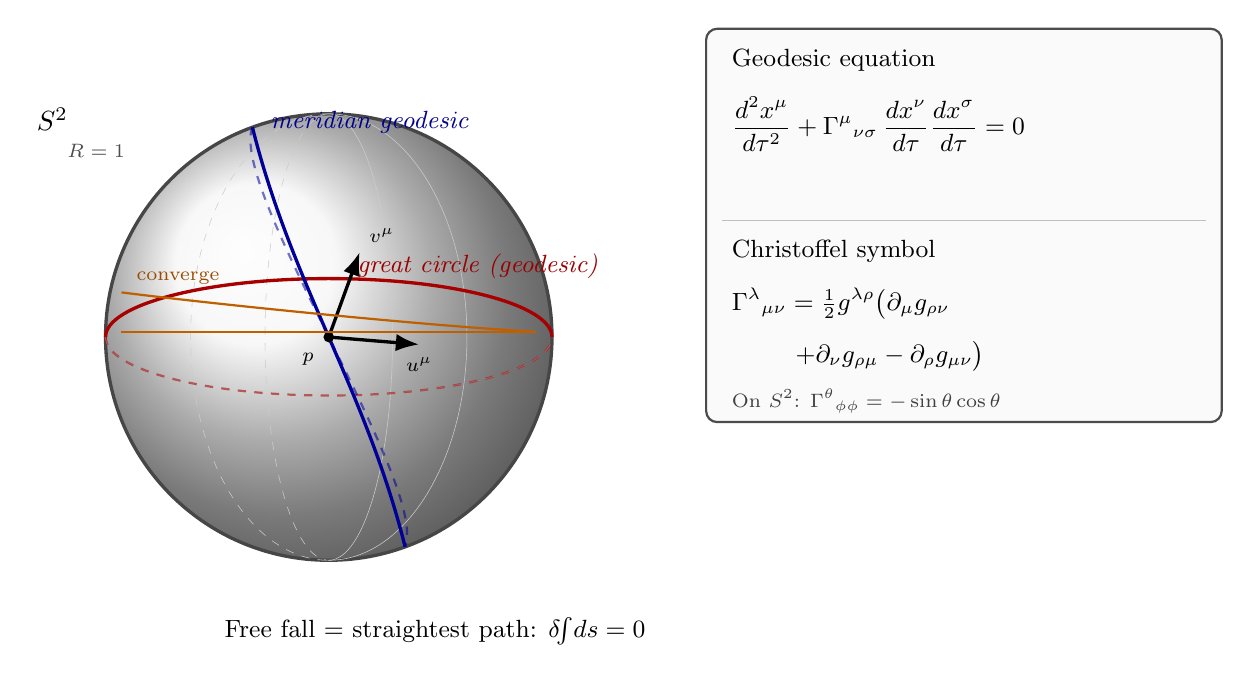
\begin{tikzpicture}[>=Latex, scale=1.35]

  % ---- Sphere body ----
  \def\R{2.1}
  \shade[ball color=gray!8] (0,0) circle (\R);
  \draw[very thick, gray!55!black] (0,0) circle (\R);

  % equator (visible front + dashed back)
  \draw[gray!50, dashed, thin]   (-\R,0) arc (180:360:{\R} and 0.55);
  \draw[gray!50, thin]           ( \R,0) arc (0:180:{\R} and 0.55);

  % a couple of meridians (dashed back / solid front)
  \draw[gray!40, dashed, very thin] (0,\R) arc (90:270:{0.6} and \R);
  \draw[gray!40, very thin]         (0,\R) arc (90:-90:{0.6} and \R);
  \draw[gray!40, dashed, very thin] (0,\R) arc (90:270:{1.3} and \R);
  \draw[gray!40, very thin]         (0,\R) arc (90:-90:{1.3} and \R);

  % ---- Geodesic 1: the equator (dark red) — front arc ----
  \draw[very thick, red!65!black] ( \R,0) arc (0:180:{\R} and 0.55);
  \draw[thick, red!65!black, dashed, opacity=0.55]
                                  (-\R,0) arc (180:360:{\R} and 0.55);

  % ---- Geodesic 2: a meridian-ish great circle through the poles (dark blue) ----
  % Tilt slightly so it crosses the equator at angle ~ 25 deg
  % Visible front semicircle:
  \draw[very thick, blue!60!black]
        ({\R*cos(110)}, {\R*sin(110)})
        .. controls ({0.55*\R*cos(110)+0.05},{0.55*\R*sin(110)-0.6})
              and  ({0.55*\R*cos(-70)-0.05},{0.55*\R*sin(-70)+0.6})
        .. ({\R*cos(-70)}, {\R*sin(-70)});
  % back half (dashed)
  \draw[thick, blue!60!black, dashed, opacity=0.55]
        ({\R*cos(110)}, {\R*sin(110)})
        .. controls ({-0.45*\R},{1.4})
              and  ({0.45*\R},{-1.4})
        .. ({\R*cos(-70)}, {\R*sin(-70)});

  % ---- Crossing point (a "pole" of these two great circles) ----
  \fill[black] (0.0, {0.55*0}) circle (0.05);
  \node[font=\scriptsize, anchor=north east] at (-0.05, -0.06) {$p$};

  % Second crossing (antipodal) marked lightly
  \fill[gray!60] (0, 0) ++(180:0) circle (0); % no-op placeholder

  % ---- Tangent vectors at p ----
  % equator tangent (rightward along equator front)
  \draw[->, very thick] (0,0) -- (0.85, -0.07);
  \node[font=\scriptsize, anchor=north] at (0.85, -0.10) {$u^\mu$};
  % second geodesic tangent at p (along blue curve direction)
  \draw[->, very thick] (0,0) -- ({0.85*cos(70)}, {0.85*sin(70)});
  \node[font=\scriptsize, anchor=south west] at ({0.85*cos(70)}, {0.85*sin(70)}) {$v^\mu$};

  % ---- Two "initially parallel" geodesics that converge: faint thin curves near equator ----
  % slightly above equator pair: starts parallel, meets near right side
  \draw[thick, orange!75!black]
        (-1.95, 0.42) .. controls (-1.0, 0.30) and (1.0, 0.10) .. (1.95, 0.05);
  \draw[thick, orange!75!black]
        (-1.95, 0.05) .. controls (-1.0, 0.05) and (1.0, 0.05) .. (1.95, 0.05);
  \node[font=\scriptsize, orange!60!black, anchor=west] at (-1.9, 0.55) {converge};

  % ---- Sphere label ----
  \node[font=\bfseries] at (-2.6, 2.05) {$S^2$};
  \node[font=\scriptsize, gray!60!black, anchor=west] at (-2.55, 1.75) {$R=1$};

  % ---- "Geodesic" label on equator ----
  \node[font=\small\itshape, red!60!black, anchor=south] at (1.4, 0.46) {great circle (geodesic)};

  % blue label
  \node[font=\small\itshape, blue!55!black, anchor=west]
        at ({\R*cos(110)+0.08}, {\R*sin(110)+0.05}) {meridian geodesic};

  % ---- Right-hand formula box ----
  \begin{scope}[shift={(3.8, 1.05)}]
    \draw[rounded corners=4pt, thick, gray!60!black, fill=gray!4]
          (-0.25, -1.85) rectangle (4.6, 1.85);

    \node[font=\small, anchor=north west] at (-0.10, 1.75)
      {Geodesic equation};

    \node[font=\small, anchor=north west] at (-0.10, 1.30)
      {$\dfrac{d^2 x^\mu}{d\tau^2}
        + \Gamma^{\mu}{}_{\nu\sigma}\,
          \dfrac{dx^\nu}{d\tau}\dfrac{dx^\sigma}{d\tau} = 0$};

    \draw[gray!50] (-0.10, 0.05) -- (4.45, 0.05);

    \node[font=\small, anchor=north west] at (-0.10, -0.05)
      {Christoffel symbol};

    \node[font=\small, anchor=north west] at (-0.10, -0.50)
      {$\Gamma^{\lambda}{}_{\mu\nu}
        = \tfrac{1}{2} g^{\lambda\rho}
        \bigl(\partial_\mu g_{\rho\nu}$};
    \node[font=\small, anchor=north west] at (0.50, -1.00)
      {$+ \partial_\nu g_{\rho\mu} - \partial_\rho g_{\mu\nu}\bigr)$};

    \node[font=\scriptsize, gray!50!black, anchor=north west] at (-0.10, -1.45)
      {On $S^2$: $\Gamma^{\theta}{}_{\phi\phi}=-\sin\theta\cos\theta$};
  \end{scope}

  % ---- Bottom caption ----
  \node[font=\small, anchor=north] at (1.0, -2.55)
    {Free fall = straightest path: $\delta\!\!\int\! ds = 0$};

\end{tikzpicture}
\end{document}
